\begin{figure}[htb]
\centering
\definecolor{seriesbuddyfree}{HTML}{2A78D6}
\definecolor{seriesbuddylargest}{HTML}{EB6834}
\definecolor{seriesring}{HTML}{2CA858}
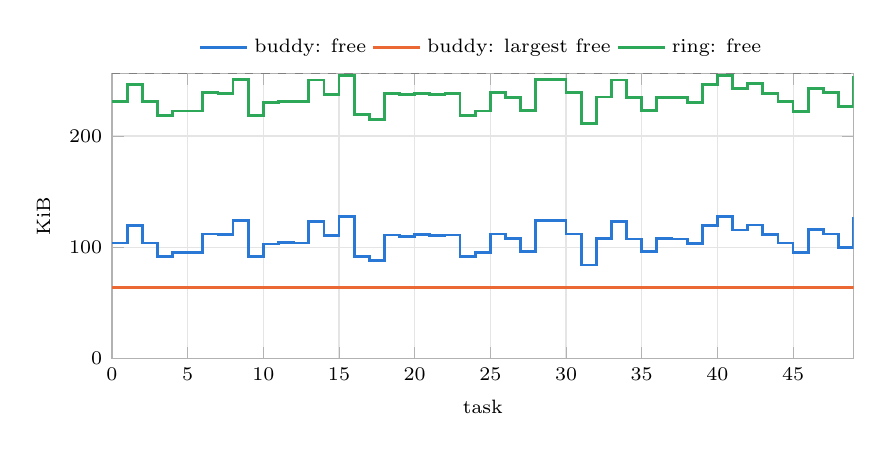
\begin{tikzpicture}
\begin{axis}[
  width=11cm, height=5.2cm,
  xlabel={task}, ylabel={KiB},
  x tick label style={font=\scriptsize}, y tick label style={font=\scriptsize},
  xlabel style={font=\scriptsize}, ylabel style={font=\scriptsize},
  xmin=0, xmax=49, ymin=0, ymax=256,
  grid=major, grid style={gray!20, thin},
  axis line style={gray!60},
  tick style={gray!60},
  const plot,
  every axis plot/.append style={line width=1pt},
  legend style={font=\scriptsize, draw=none, fill=none, at={(0.5,1.02)}, anchor=south, legend columns=3},
]
\addplot[color=gray, dashed, mark=none, line width=0.5pt, forget plot] coordinates {(0,256) (49,256)};
\addplot[color=seriesbuddyfree, mark=none] coordinates {
  (0,103.94) (1,119.38) (2,103.94) (3,91.44) (4,95.50) (5,95.50) (6,111.94) (7,111.44) (8,123.94) (9,91.50)
  (10,103.00) (11,104.00) (12,103.88) (13,123.38) (14,110.44) (15,127.44) (16,92.00) (17,87.94) (18,110.94)
  (19,110.00) (20,111.44) (21,110.50) (22,111.00) (23,91.50) (24,95.44) (25,111.94) (26,107.94) (27,95.94)
  (28,123.75) (29,123.94) (30,111.94) (31,84.00) (32,108.00) (33,123.38) (34,107.44) (35,96.00) (36,107.94)
  (37,107.44) (38,103.44) (39,119.44) (40,127.44) (41,115.50) (42,120.00) (43,111.44) (44,103.94) (45,95.38)
  (46,115.94) (47,111.94) (48,99.50) (49,126.94)
};
\addplot[color=seriesbuddylargest, mark=none] coordinates {
  (0,64.00) (1,64.00) (2,64.00) (3,64.00) (4,64.00) (5,64.00) (6,64.00) (7,64.00) (8,64.00) (9,64.00)
  (10,64.00) (11,64.00) (12,64.00) (13,64.00) (14,64.00) (15,64.00) (16,64.00) (17,64.00) (18,64.00)
  (19,64.00) (20,64.00) (21,64.00) (22,64.00) (23,64.00) (24,64.00) (25,64.00) (26,64.00) (27,64.00)
  (28,64.00) (29,64.00) (30,64.00) (31,64.00) (32,64.00) (33,64.00) (34,64.00) (35,64.00) (36,64.00)
  (37,64.00) (38,64.00) (39,64.00) (40,64.00) (41,64.00) (42,64.00) (43,64.00) (44,64.00) (45,64.00)
  (46,64.00) (47,64.00) (48,64.00) (49,64.00)
};
\addplot[color=seriesring, mark=none] coordinates {
  (0,230.91) (1,246.34) (2,230.91) (3,218.41) (4,222.47) (5,222.47) (6,238.91) (7,238.41) (8,250.91) (9,218.47)
  (10,229.97) (11,230.97) (12,230.84) (13,250.34) (14,237.41) (15,254.41) (16,218.97) (17,214.91) (18,237.91)
  (19,236.97) (20,238.41) (21,237.47) (22,237.97) (23,218.47) (24,222.41) (25,238.91) (26,234.91) (27,222.91)
  (28,250.72) (29,250.91) (30,238.91) (31,210.97) (32,234.97) (33,250.34) (34,234.41) (35,222.97) (36,234.91)
  (37,234.41) (38,230.41) (39,246.41) (40,254.41) (41,242.47) (42,246.97) (43,238.41) (44,230.91) (45,222.34)
  (46,242.91) (47,238.91) (48,226.47) (49,253.91)
};
\legend{buddy: free, buddy: largest free, ring: free}
\end{axis}
\end{tikzpicture}
\caption{Free space in a buddy and a ring allocator during each of 50
tasks, sampled just before each task frees everything. Both are built on a
256\,KiB region (dashed line), and the closer a line stays to it, the more room is
left. Ring's largest free block equals its total
free space (green) in every task, so only one line is drawn for it. The
minimums are in \cref{tab:temp-buddy}. One run with a fixed seed, as in
\cref{tab:arena-vs-buddy}.}
\label{fig:temp-buddy-series}
\end{figure}
